\documentclass{article} % For LaTeX2e
\pdfoutput=1 % for arxiv to accept pdf figures
\usepackage[utf8]{inputenc}
\usepackage{nips15submit_e,times}
\usepackage{hyperref}
\usepackage{graphicx}
\usepackage{subfigure}
\usepackage{hyperref}
\usepackage{url}
\usepackage{times}
\usepackage{epsfig}
\usepackage{graphicx}
\usepackage{amsmath}
\usepackage{amssymb}
\usepackage{multirow}
\usepackage{caption}
\usepackage{minipage} 
\usepackage{url}
\usepackage{booktabs}
\renewcommand{\arraystretch}{1.2}
%\documentstyle[nips14submit_09,times,art10]{article} % For LaTeX 2.09

\title{Recurrent Batch Normalization}

\author{
Tim Cooijmans$^\dagger$ \\
\And
Nicolas Ballas$^\star$ \\
\And
C\'esar Laurent$^\star$ \\
\And
Çağlar Gülçehre$^\star$ \\
\And
Aaron Courville$^\star$\\
MILA - Universit\'e de Montr\'eal\\
$^\dagger$ \texttt{lastname.firstname@gmail.com} \\
$^\star$ \texttt{firstname.lastname@umontreal.ca} \\
}

\newcommand{\fix}{\marginpar{FIX}}
\newcommand{\new}{\marginpar{NEW}}

\nipsfinalcopy % Uncomment for camera-ready version

\usepackage{amsfonts}
\usepackage{amsmath}

\newcommand{\vect}[1]{\mathbf{#1}}
\newcommand{\mat}[1]{\mathbf{#1}}
\newcommand{\act}{f}
\newcommand{\ewprod}{\odot}
\newcommand{\reals}{\mathbb{R}}
\newcommand{\given}{\vert}

\bibliographystyle{plain}

\begin{document}

\maketitle

\begin{abstract}
We propose a reparameterization of LSTM that brings the benefits of batch normalization to recurrent neural networks.
Whereas previous works only apply batch normalization to the input-to-hidden transformation of RNNs,
we demonstrate that it is both possible and beneficial to batch-normalize the hidden-to-hidden transition,
thereby reducing internal covariate shift between time steps.

We evaluate our proposal on various sequential problems such as sequence classification, language modeling and question answering.
Our empirical results show that our batch-normalized LSTM consistently leads to faster convergence and improved generalization.
\end{abstract}

\section{Introduction}

Recurrent neural network architectures such as LSTM~\cite{lstm} and GRU~\cite{cho2014learning} have recently exhibited
state-of-the-art performance on a wide range of complex sequential problems including speech recognition~\cite{baidu},
machine translation~\cite{bahdanau2014neural} and image and video captioning~\cite{xu2015show,yao2015describing}.
Top-performing models, however, are based on very high-capacity networks that are computationally intensive and costly to train.
Effective optimization of recurrent neural networks is an active area of study~\cite{pascanudifficulty,hessianfree,ollivier}.

It is known that for deep feed-forward neural networks, covariate shift~\cite{shimodaira2000improving,batchnorm}
degrades the efficiency of training.
Covariate shift is a change in distribution of the inputs to a model.
This occurs continuously during training of feed-forward neural networks,
where changing the parameters of a layer affects the distribution of the inputs to all layers above it.
As a result, the upper layers are continually adapting to the shifting input distribution and unable to learn effectively.
This \emph{internal} covariate shift~\cite{batchnorm} may play an especially important role in recurrent neural networks,
which resemble very deep feed-forward networks.

Batch normalization~\cite{batchnorm} is a recently proposed technique for controlling the distributions of feed-forward neural network activations, thereby reducing internal covariate shift.
It involves standardizing the activations going into each layer, enforcing their means and variances to be invariant to changes in the parameters of the underlying layers.
% relying on the observation that a network converges faster when its inputs have zero mean, unit variance and are uncorrelated~\cite{efficientbackprop}.
This effectively decouples each layer's parameters from those of other layers, leading to a better-conditioned optimization problem.
Indeed, deep neural networks trained with batch normalization converge significantly faster and generalize better.

Although batch normalization has demonstrated significant training speed-ups and generalization benefits in feed-forward networks,
it has proven difficult to apply in recurrent architectures~\cite{cesar,baidu}.
It has found limited use in stacked RNNs, where the normalization is applied ``vertically'',
i.e. to the input of each RNN, but not ``horizontally'' between timesteps.
RNNs are deepest in the time direction, and as such batch normalization would be most beneficial when applied horizontally.
However, it has been hypothesized~\cite{cesar} that applying batch normalization in this way hurts training
because of exploding gradients due to repeated rescaling.

Our findings run counter to this hypothesis.
We show that it is both possible and highly beneficial to apply batch normalization in the hidden-to-hidden transition of recurrent models.
In particular, we describe a reparameterization of LSTM that involves batch normalization
and demonstrate that doing so speeds up optimization and improves generalization.
In addition, we empirically analyze the gradient backpropagation and show that proper initialization
of the batch normalization parameters is crucial to avoiding vanishing gradient.

We evaluate our proposal on several sequential problems and show that our
LSTM reparameterization consistently outperforms the LSTM baseline across tasks,
in terms of both time to convergence and performance.
In particular, we achieve state-of-the-art performance on
Sequential MNIST~\cite{le2015simple} and
character-level language modeling on the text8~\cite{mahoney2009large} corpus.

%% FIXME add section 4
Section~\ref{sec:prerequisites} introduces RNNs and batch normalization in detail.
In Section~\ref{sec:recurrent-batch-normalization}, we discuss batch normalization in the recurrent setting.
Section~\ref{sec:activation-variance} investigates the impact of the batch normalization scale parameter on the gradient back-propagation for
recurrent models. We show in Section~\ref{sec:experiments} our evaluation
of the proposed reparameterization on a variety of tasks.

\section{Prerequisites}
\label{sec:prerequisites}


\subsection{LSTM}

Long Short-Term Memory (LSTM) networks are an instance of a more general class of recurrent neural networks (RNNs),
which we shall briefly review.
Given an input sequence $\mat{X} = ( \vect{x}_1, \vect{x}_2, \ldots, \vect{x}_T )$,
an RNN defines a sequence of hidden states $h_t$ according to
\begin{eqnarray}
  \mat{h}_t = \phi(\mat{W}_h \vect{h}_{t-1} + \mat{W}_x  \vect{x}_t + \vect{b}),
\end{eqnarray}
where $\mat{W}_h \in \reals^{d_h \times d_h}, \mat{W}_x \in \reals^{d_x \times d_h}, \vect{b} \in \reals^{d_h}$
and the initial state $\vect{h}_0 \in \reals^{d_h}$ % I've put this back because I believe we do need to say something about the initial state -- tim
are model parameters.
A popular choice for the activation function $\phi(\ \cdot\ )$ is $\tanh$.

RNNs are popular in sequence modeling because of their natural ability to process variable-length sequences.
Training RNNs using first-order stochastic gradient descent (SGD) however is notoriously difficult
due to the well-known problem of exploding/vanishing gradients~\cite{bengio1994learning,hochreiter1991untersuchungen,pascanudifficulty}.
Gradient vanishing occurs when states $h_t$ are not influenced by small changes in much earlier states $h_{\tau}$, $t \ll \tau$,
preventing learning of long-term dependencies in the input data.
While the long-term dependencies problem is unsolvable in absolute~\cite{bengio1994learning},
it has been demonstrated that different RNN reparameterizations, such as the LSTM~\cite{lstm}, GRU~\cite{cho2014learning} or $i$/$u$-RNN~\cite{le2015simple,urnn}
can help mitigate the vanishing gradient problem.

In what follows, we focus on the LSTM architecture~\cite{lstm} with recurrent transition given by
\begin{eqnarray}
\left(\begin{array}{ccc}
\tilde{\vect{f}}_t \\
\tilde{\vect{i}}_t \\
\tilde{\vect{o}}_t \\
\tilde{\vect{g}}_t
\end{array}\right)
 &=&
 \mat{W}_h \vect{h}_{t-1} +
 \mat{W}_x \vect{x}_t +
 \vect{b}
 \\
\vect{c}_t &= &\sigma(\tilde{\vect{f}}_t) \ewprod \vect{c}_{t-1} +
\sigma(\tilde{\vect{i}}_t) \ewprod \tanh(\tilde{\vect{g}_t}) \\
\vect{h}_t &= &\sigma(\tilde{\vect{o}}_t) \ewprod \tanh(\vect{c}_t),
\end{eqnarray}
where $\vect{W}_h \in \reals^{d_h \times 4 d_h}, \vect{W}_x \reals^{d_x \times 4 d_h}, \vect{b} \in \reals^{4 d_h}$
and the initial states $\vect{h}_0 \in \reals^{d_h}, \vect{c}_0 \in \reals^{d_h}$ % I've put this back because I believe we do need to say something about the initial state -- tim
are model parameters.
$\sigma$ is the logistic sigmoid function, and the $\ewprod$ operator denotes the Hadamard product.

The LSTM differs from simple RNNs in that it has an additional memory \emph{cell} 
$\vect{c}_t$ whose update is nearly linear which allows the gradient to flow back 
through time more easily. In addition, unlike the RNN which overwrites its content 
at each timestep, the update of the LSTM cell is regulated by a set of gates.
The forget gate $\vect{f}_t$ determines the extent to which information is carried over from the previous timestep,
and the input gate $\vect{i}_t$ controls the flow of information from the current input $\vect{x}_t$.
The output gate $\vect{o}_t$ allows the model to read from the cell. This carefully 
controlled interaction with the cell is what allows the LSTM to robustly retain 
information for long periods of time.

\subsection{Batch Normalization}

\emph{Covariate shift}~\cite{shimodaira2000improving} is a phenomenon in machine learning where
the features presented to a model change in distribution during the course of training.
In order for learning to succeed in the presence of covariance shift,
the model's parameters must be adjusted not just to learn the concept at hand
but also to adapt to the changing distribution of the inputs.
In deep neural networks, this problem manifests as \emph{internal covariance shift}~\cite{batchnorm},
where changing the parameters of a layer affects the distribution of the inputs to all layers above it.

Batch Normalization~\cite{batchnorm} is a recently proposed network reparameterization that aims to reduce internal covariate shift.
It does so by standardizing the activations using statistical estimates of their means and standard deviations.
However, it does not decorrelate the activations as the matrix inversion involved would be too expensive.

The batch normalizing transform is as follows:

\begin{align}
\mathrm{BN}(\vect{h}; \gamma, \beta) =
  \beta + \gamma
  \frac{\vect{h} -   \widehat{\mathbb{E  }}(\vect{h})}
       {       \sqrt{\widehat{\mathrm{Var}}(\vect{h}) + \epsilon}}
\end{align}

where $\vect{h} \in \reals^d$ is the vector of (pre)activations to be normalized, 
$\gamma \in \reals^d, \beta \in \reals^d$ are model parameters that determine the 
mean and standard deviation of the normalized activation, and $\epsilon \in \reals$ 
is a regularization hyperparameter. The division should be understood to proceed elementwise.

At training time, the statistics $\mathbb{E}(\vect{h})$ and $\mathrm{Var}(\vect{h})$ are estimated
by the sample mean and sample variance of the current minibatch.
This allows for backpropagation through the statistics, preserving the convergence properties of stochastic gradient descent.
During inference, the statistics are typically estimated based on the entire training set, so as to produce a deterministic prediction.

\begin{figure}[!ht]
\center
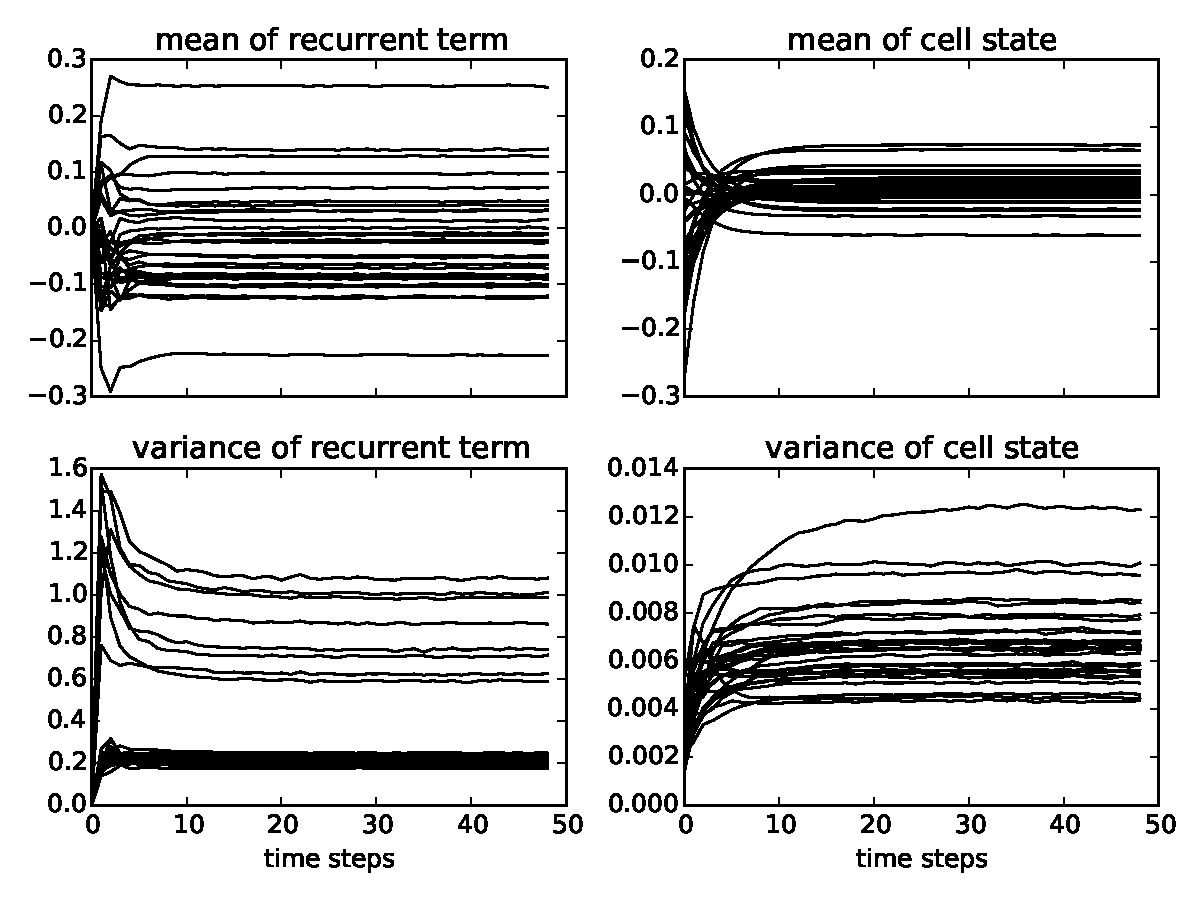
\includegraphics[width=0.8\textwidth]{figures/popstat_stationarity.pdf}
\caption{Convergence of population statistics to stationary distributions on the 
Penn Treebank task. Only a random subset of population statistics is shown.}
\label{fig:popstat_stationarity}
\end{figure}



\section{Batch-Normalized LSTM}
\label{sec:recurrent-batch-normalization}

This section introduces a reparameterization of LSTM that takes advantage of 
batch normalization. Contrary to previous work~\cite{cesar, baidu}, we 
leverage batch normalization in both the input-to-hidden \emph{and} the hidden-to-hidden transformations.
We introduce the batch-normalizing transform $\mathrm{BN}(\ \cdot\ ; \gamma, \beta)$ 
into the LSTM as follows:

\begin{eqnarray}
\left(\begin{array}{ccc}
\tilde{\vect{f}}_t \\
\tilde{\vect{i}}_t \\
\tilde{\vect{o}}_t \\
\tilde{\vect{g}}_t
\end{array}\right)
 &=&
 \mathrm{BN} (\mat{W}_h \vect{h}_{t-1}; \gamma_h, \beta_h) +
 \mathrm{BN} (\mat{W}_x \vect{x}_t   ; \gamma_x, \beta_x) +
 \vect{b}
\\
\vect{c}_t &=& \sigma(\tilde{\vect{f}}_t) \ewprod \vect{c}_{t-1} +
               \sigma(\tilde{\vect{i}}_t) \ewprod \tanh(\tilde{\vect{g}_t}) \\
\vect{h}_t &=& \sigma(\tilde{\vect{o}}_t) \ewprod \tanh(
 \mathrm{BN} (\vect{c}_t; \gamma_c, \beta_c)
)
\end{eqnarray}



In our formulation, we normalize the recurrent term $\mat{W}_h \vect{h}_{t-1}$ and the input term $\mat{W}_x \vect{x}_t$ separately.
Normalizing these terms individually gives the model better control over the relative contribution of the terms using the $\gamma_h$ and $\gamma_x$ parameters.
We set $\beta_h = \beta_x = \vect{0}$ to avoid unnecessary redundancy, instead relying on the pre-existing parameter vector $\vect{b}$ to account for both biases.
In order to leave the LSTM dynamics intact and preserve the gradient flow through $\vect{c}_t$, we do not apply batch normalization on the cell states.


The batch normalization transform relies on batch statistics to standardize the LSTM activations.
It would seem natural to share the statistics that are used for normalization across time,
just as recurrent neural networks share their parameters over time.
However, we have found that simply averaging statistics over time severely degrades performance.
Although LSTM activations do converge to a stationary distribution, we have empirically observed that their statistics during the initial transient differ significantly as figure~\ref{fig:popstat_stationarity} shows.
Consequently, we recommend using separate statistics for each timestep to preserve
information of the initial transient phase in the activations.

Generalizing the model to sequences longer than those seen during training
is straightforward thanks to the rapid convergence of the activations
to their steady-state distributions (cf. Figure~\ref{fig:popstat_stationarity}).
For our experiments we estimate the population statistics separately for each timestep $1, \ldots, T_{max}$ where $T_{max}$ is the length of the longest training sequence.
When at test time we need to generalize beyond $T_{max}$, we use the population statistic of time $T_{max}$ for all time steps beyond it.

During training we estimate the statistics across the minibatch, independently for each timestep.
At test time we use estimates obtained by averaging the minibatch estimates over the training set.


%% [there is an annoying little detail here: there may be only a single example with length T, and so the population statistic is highly unreliable. in this case i would take an earlier population statistic instead, the exact choice determined by validation. how do we explain this concisely?]
%% [additionally, we haven't actually dealt with variable-length training sequences yet. this is another technicality that's easily hacked around but people will want to know i guess.]


\section{Initializing $\gamma$ for Gradient Flow}
\label{sec:activation-variance}

\begin{figure}[!ht]
  \center%
  \subfigure[
Gradient flow through a batch-normalized $\tanh$ RNN as a function of $\gamma$.
High variance causes vanishing gradient.
]{%
    \label{fig:rnn_grad_prop}
    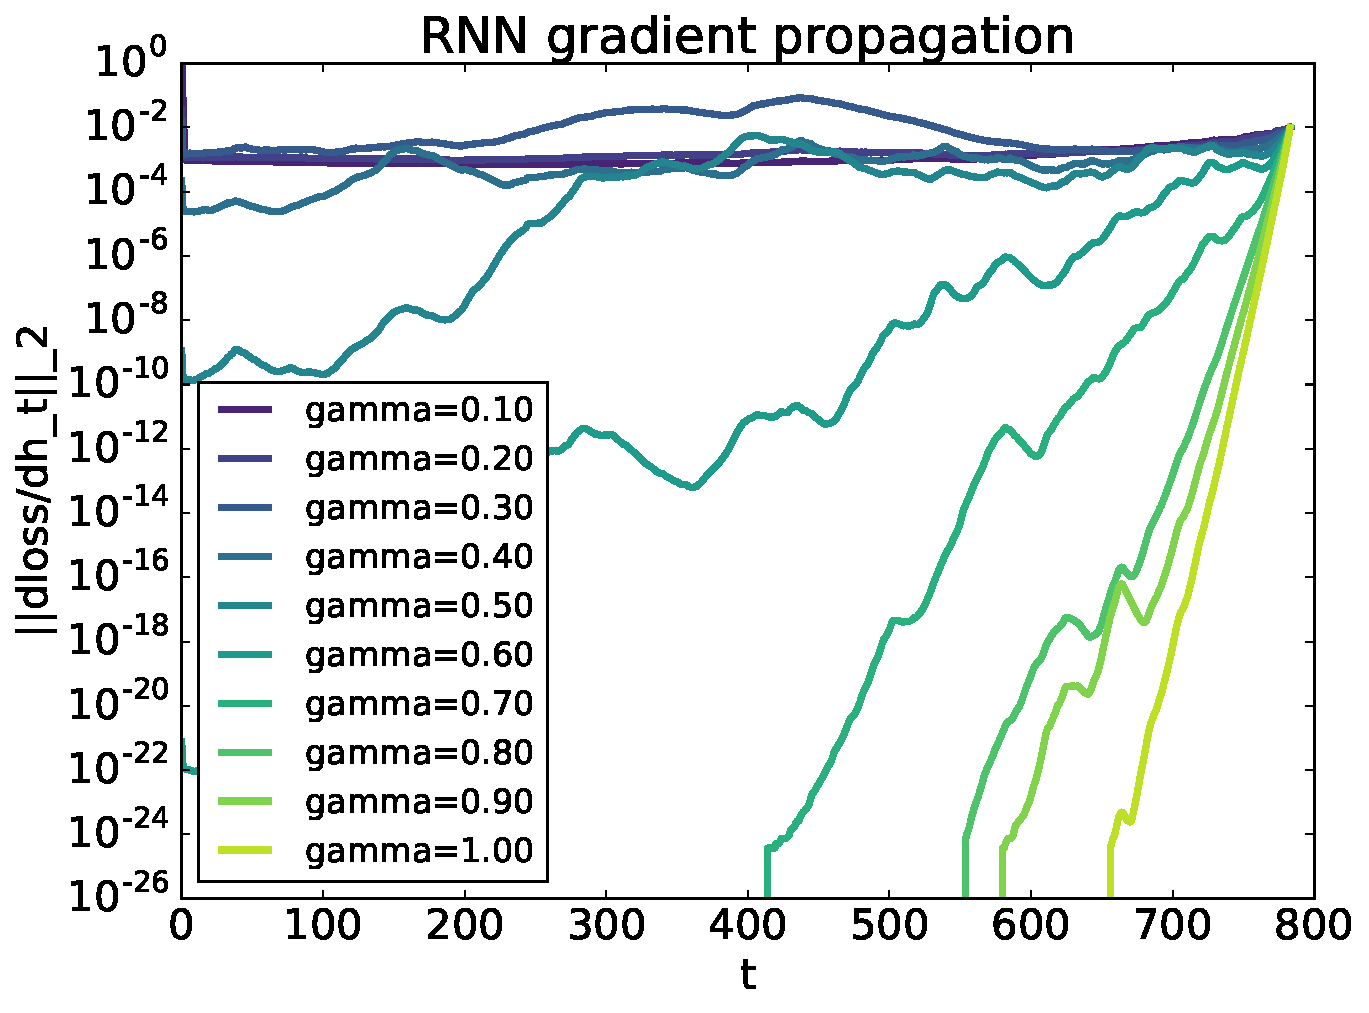
\includegraphics[width=.45\textwidth]{figures/rnn_grad_prop.pdf}
  }%
  \hspace{2mm}%
  \subfigure[
Empirical expected derivative of $\tanh$ nonlinearity as a function of input variance.
High variance causes saturation, which decreases the expected derivative.
]{%
    \label{fig:tanh_grad}
    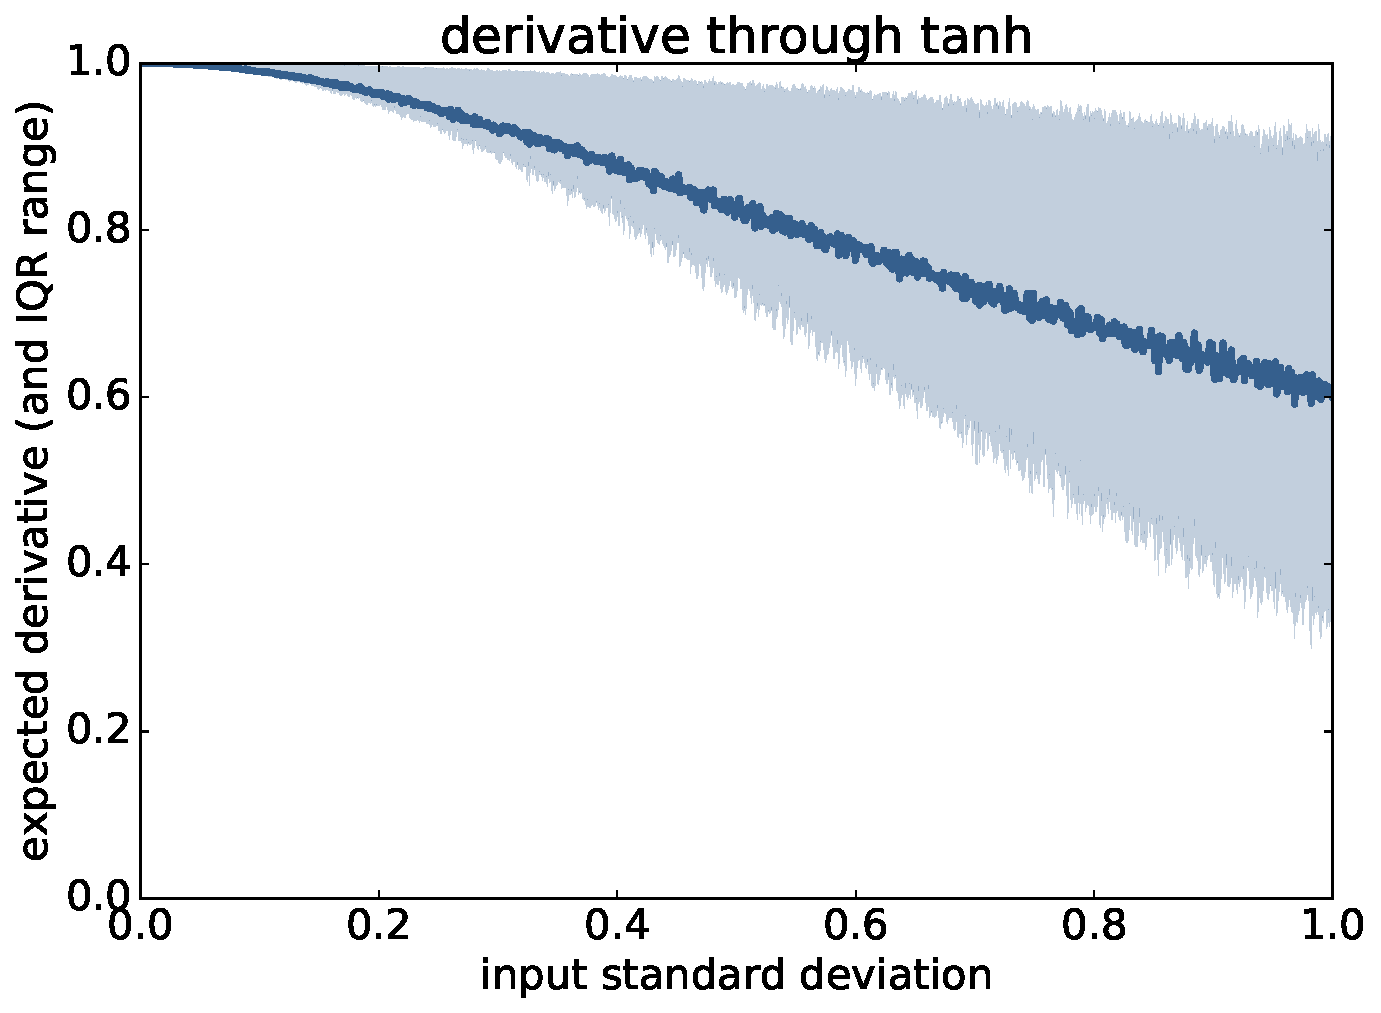
\includegraphics[width=.45\textwidth]{figures/tanh_grad.pdf}
  }
  \caption{
Influence of pre-activation variance on gradient propagation.
}
  \label{fig:variance}
\end{figure}

Although batch normalization allows for easy control of the pre-activation variance through the $\gamma$ parameters,
common practice is to normalize to unit variance.
We suspect that the previous difficulties with recurrent batch normalization reported in the literature~\cite{cesar,baidu}
are largely due to improper initialization of the batch normalization parameters, and $\gamma$ in particular.
In this section we demonstrate the impact of $\gamma$ on gradient flow.

In Figure~\ref{fig:rnn_grad_prop} we show how the pre-activation variance impacts gradient propagation in a simple RNN on the sequential MNIST task described in Section~\ref{sec:seqmnist}.
Since backpropagation operates in reverse, the plot is best read from right to left.
The quantity plotted is the norm of the gradient of the loss with respect to the hidden state at different time steps.
For large values of $\gamma$, the norm quickly goes to zero as gradient is propagated back in time.
For small values of $\gamma$ the norm is nearly constant.

Figure~\ref{fig:tanh_grad} shows empirically how the expected derivative of the $\tanh$ nonlinearity changes with the variance of the argument.
When the input variance is low, the input tends to be close to the origin where the derivative is close to 1.
As the variance increases, the expected derivative decreases as the input is more likely to be in the saturation regime.
At unit variance, the expected derivative is much smaller than 1.

We conjecture that this is what causes the gradient to vanish, and recommend initializing $\gamma$ to a small value.
In our trials we found that values of 0.01 or lower caused instabilities during training.
Our choice of 0.1 seems to work well across tasks.

\section{Experiments}
\label{sec:experiments}

This section presents an empirical evaluation of the proposed batch-normalized LSTM on four different tasks. Results show that batch-normalized LSTM achieves convergence faster than a baseline LSTM on all the tasks, and, can also lead to better generalization.

Note that for all the experiments, we initialize the batch normalization scale and shift parameters $\gamma$ and $\beta$ to $0.1$ and $0$ respectively.



\subsection{Sequential MNIST}
\label{sec:seqmnist}

\begin{figure}
\center
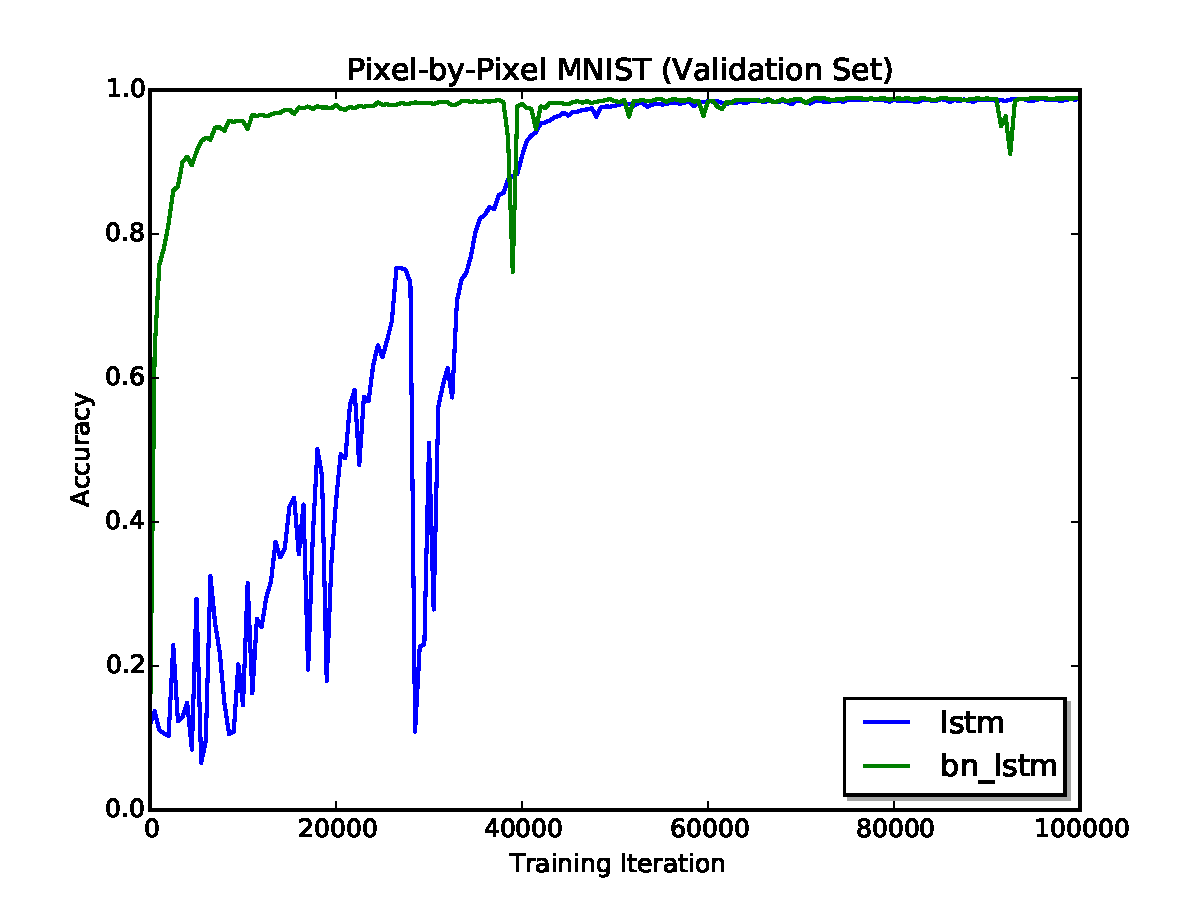
\includegraphics[width=6.7cm]{figures/unpermuted_valid.pdf}
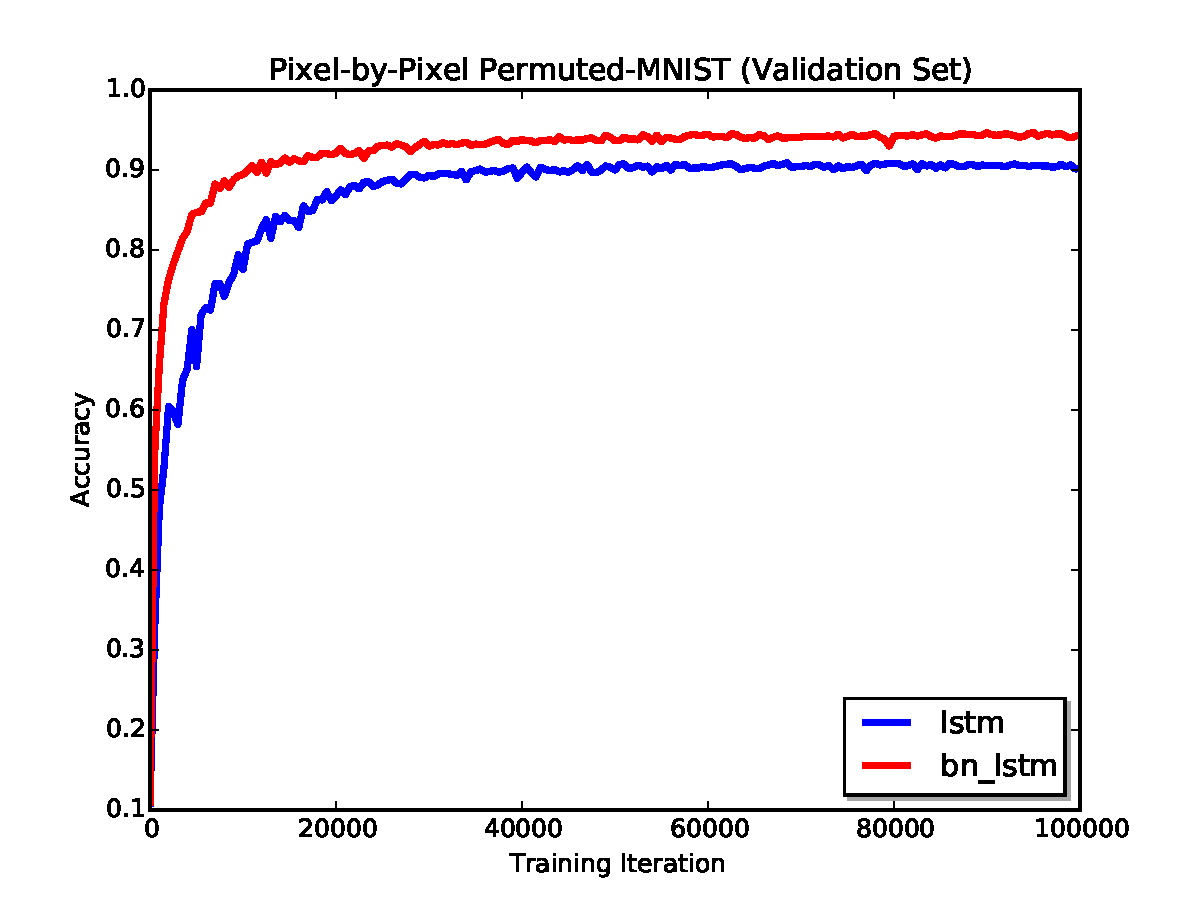
\includegraphics[width=6.7cm]{figures/permuted_valid.pdf}
\caption{Accuracy on the validation set for the pixel by pixel MNIST classification tasks. The batch-normalized LSTM is able to converge faster relatively to a baseline LSTM.
  Batch-normalized  LSTM also shows some improve generalization on the permuted sequential MNIST that require to preserve long-term memory information.}
\label{fig:seqmnist_valid}
\end{figure}


We evaluate our batch-normalized LSTM on a sequential version of the MNIST classification task~\cite{le2015simple}.
The model processes each image one pixel at a time and finally predicts the label.
We consider both sequential MNIST tasks, MNIST and permuted MNIST ($p$MNIST).
In MNIST, the pixels are processed from left to right, top to bottom.
In $p$MNIST the pixels are processed in a fixed random order.

Our baseline consists of an LSTM with 100 hidden units, with a softmax classifier to produce a prediction from the final hidden state.
We use orthogonal initialization for all weight matrices, except for the hidden-to-hidden weight matrix which we initialize to be the identity matrix,
as this yields better generalization performance on this task for both models.
The model is trained using RMSProp~\cite{rmsprop} with learning rate of $10^{-3}$ and $0.9$ momentum.
We apply gradient clipping at 1 to avoid exploding gradients.

The in-order MNIST task poses a unique problem for our model:
the input for the first hundred or so timesteps is constant across examples since the upper pixels are almost always black.
This causes the variance of the hidden states to be exactly zero for a long period of time.
Normalizing these zero-variance activations involves division by a small number at many timesteps, which causes the gradient to explode.
We work around this by injecting noise into the initial hidden states.
Although the normalization amplifies the noise to signal level, we find that it does not hurt performance compared to data-dependent ways of initializing the hidden states.
%[but is that an artifact of classification at the end?]


\begin{table}
\center
\begin{tabular}{@{}lcc@{}}
  \toprule
  \bf Model & \bf MNIST & \bf $p$MNIST \\
  \midrule
  TANH-RNN~\cite{le2015simple} & 35.0 & 35.0\\
  $i$RNN~\cite{le2015simple} & 97.0 & 82.0\\
  $u$RNN~\cite{urnn} & 95.1 & 91.4\\
  $s$TANH-RNN~\cite{zhang2016architectural} & 98.1 & 94.0\\
  \midrule
  LSTM (ours) & 98.9 & 90.2\\
  BN-LSTM (ours) & \textbf{99.0} & \textbf{95.4}\\
  \bottomrule
\end{tabular}
\caption{Accuracy obtained on the test set for the pixel by pixel MNIST classification tasks}
\label{tab:seqmnist_test}

\end{table}

In Figure~\ref{fig:seqmnist_valid} we show the validation accuracy while training for both LSTM and batch-normalized LSTM (BN-LSTM).
BN-LSTM converges faster than LSTM on both tasks.
Additionally, we observe that BN-LSTM generalizes significantly better on $p$MNIST.
It has been highlighted in~\cite{urnn} that
$p$MNIST contains many longer term dependencies across pixels than in
the original pixel ordering, where a lot of structure is local.
A recurrent network therefore needs to characterize dependencies across varying time scales in order to solve this tasks.
Our results suggest that BN-LSTM is better able to capture these long-term dependencies.

Table~\ref{tab:seqmnist_test} reports the test set accuracy of the early stop model for LSTM and BN-LSTM using the population statistics.
Recurrent batch normalization leads to better test score, especially for $p$MNIST where models have to leverage long-term temporal depencies.
In addition, Table~\ref{tab:seqmnist_test} shows that our batch-normalized LSTM achieves state of the art on both MNIST and $p$MNIST.

\subsection{Character-level Penn Treebank}

\begin{figure}
  \center%
  \subfigure[
    Performance in bits-per-character on length-100 subsequences of the Penn Treebank
    validation sequence during training.
]{%
    \label{fig:ptb_valid}
    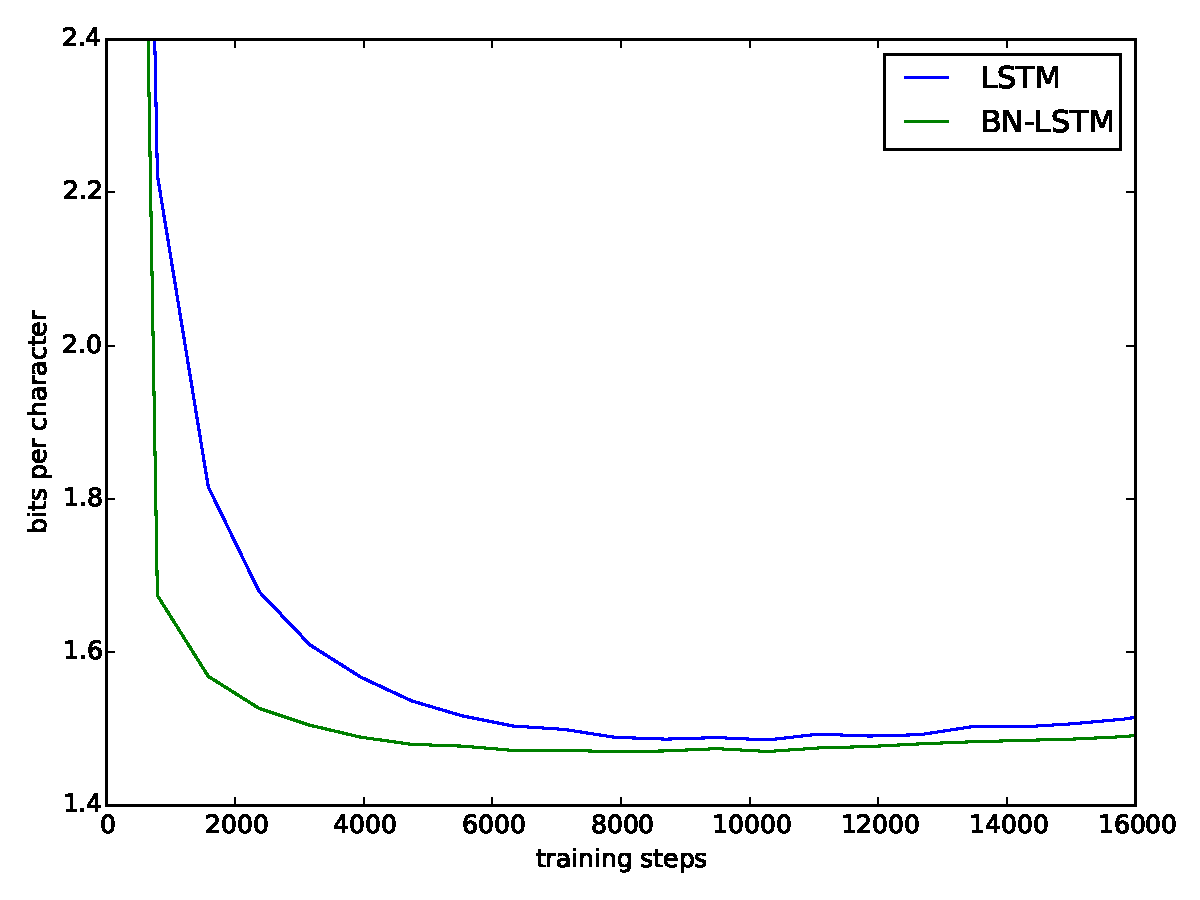
\includegraphics[width=.45\textwidth]{figures/ptb_valid.pdf}
  }%
  \hspace{2mm}%
  \subfigure[
    Generalization to longer subsequences of Penn Treebank using population statistics.
    The subsequences are taken from the test sequence.
]{%
    \label{fig:ptb_lengths}
    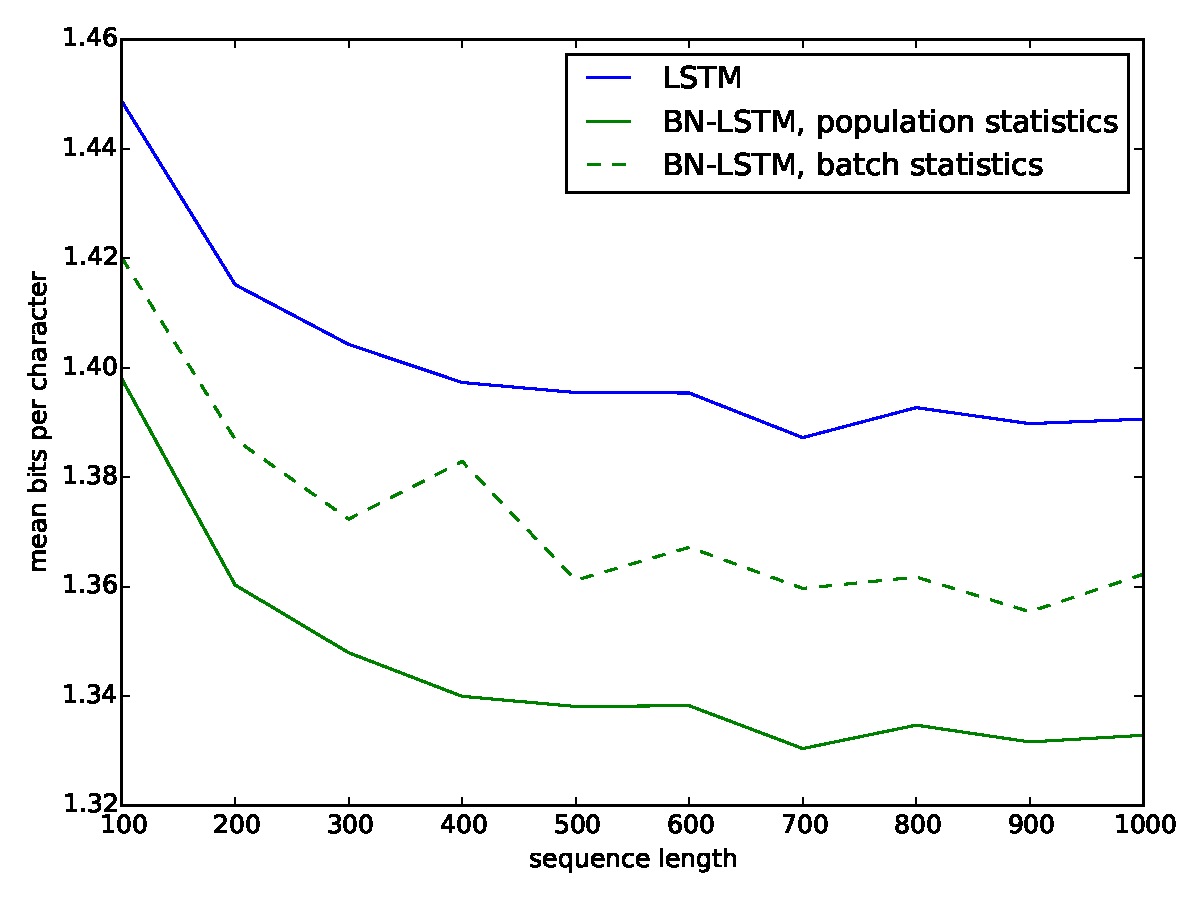
\includegraphics[width=.45\textwidth]{figures/ptb_lengths.pdf}
  }
  \caption{Penn Treebank evaluation}
  \label{fig:ptb}
\end{figure}

\begin{table}
  \center
\begin{minipage}[t]{6.5cm}
\begin{tabular}{@{}lc@{}}
  \toprule
  \bf Model & \bf Penn Treebank \\
  \midrule
  LSTM~\cite{graves2013generating} &  1.26\footnote{Our performance does not directly compare against~\cite{graves2013generating} as they use a different dataset split.}\\
  \midrule
  HF-MRNN~\cite{mikolov2012subword} & 1.41 \\
  Norm-stabilized LSTM~\cite{krueger} & 1.39 \\
  ME n-gram~\cite{mikolov2012subword} & 1.37 \\
  \midrule
  LSTM (ours) & 1.38 \\
  BN-LSTM (ours) & 1.32 \\
  \bottomrule
\end{tabular}
\caption{Bits-per-character on the Penn Treebank test sequence.}
\label{tab:ptb_test}
\end{minipage}
\hspace{1cm}
\begin{minipage}[t]{4.5cm}
  \begin{tabular}{@{}lc@{}}
  \toprule
  \bf Model & \bf text8 \\
  \midrule
  $td$-LSTM~\cite{zhang2016architectural} & 1.63 \\
  HF-MRNN~\cite{mikolov2012subword} & 1.54 \\
  skipping RNN~\cite{pachitariu2013regularization} & 1.48 \\
  \midrule
  LSTM (ours) &  1.41 \\
  BN-LSTM (ours) & \textbf{1.39} \\
  \bottomrule
\end{tabular}
\caption{Bits-per-character on the text8 test sequence.}
\label{tab:text8_test}
\end{minipage}
\end{table}


We evaluate our model on the task of character-level language modeling on the Penn Treebank corpus~\cite{penntreebank}
according to the train/valid/test partition of~\cite{mikolov2012subword}.
For training, we segment the training sequence into examples of length 100.
The training sequence does not cleanly divide by 100, so for each epoch we randomly crop a subsequence that does and segment that instead.

Our baseline is an LSTM with 1000 units, trained to predict the next character using a softmax classifier on the hidden state $h_t$.
We use stochastic gradient descent on minibatches of size 64,
with gradient clipping at 1.0 and step rule determined by Adam~\cite{kingma2014adam}
with learning rate 0.002.
We use orthogonal initialization for all weight matrices.
The setup for the batch-normalized LSTM is the same in all respects except for the introduction of batch normalization as detailed in~\ref{sec:recurrent-batch-normalization}.

We show the learning curves in Figure~\ref{fig:ptb_valid}.
BN-LSTM converges faster and generalizes better than the LSTM baseline.
Figure~\ref{fig:ptb_lengths} shows the generalization of our model to longer sequences.
We observe that using the population statistics improves generalization performance,
which confirms that repeating the last population statistic (cf. section~\ref{sec:recurrent-batch-normalization})
is a viable strategy.
In table~\ref{tab:ptb_test} we report the performance of our best models (early-stopped on validation performance)
on the Penn Treebank test sequence and compare them to previous work.
It shows that our BN-LSTM model compares favorably to state-of-the-art models.



\subsection{Text8}

We evaluate our model on a second character-level language modeling task on the text8 dataset~\cite{mahoney2009large}.
This dataset is derived from Wikipedia and consists of a sequence of 100M characters including only alphabetical characters and spaces.
We follow previous authors~\cite{mikolov2012subword,zhang2016architectural} and use the first 90M characters for training, the next 5M for validation and the final 5M characters for testing.
We train on nonoverlapping sequences of length 180.

Our model is a BN-LSTM with 2000 units, trained to predict the next character using a softmax classifier on the hidden state $h_t$.
We use stochastic gradient descent on minibatches of size 64,
with gradient clipping at 1.0 and step rule determined by Adam~\cite{kingma2014adam}
with learning rate 0.01.
All weight matrices were initialized to be orthogonal.

We early-stop on validation performance and report the test performance of the resulting model in table~\ref{tab:text8_test}.
Our model achieves state of the art.

\subsection{Teaching Machines to Read and Comprehend}

\begin{figure}
\center
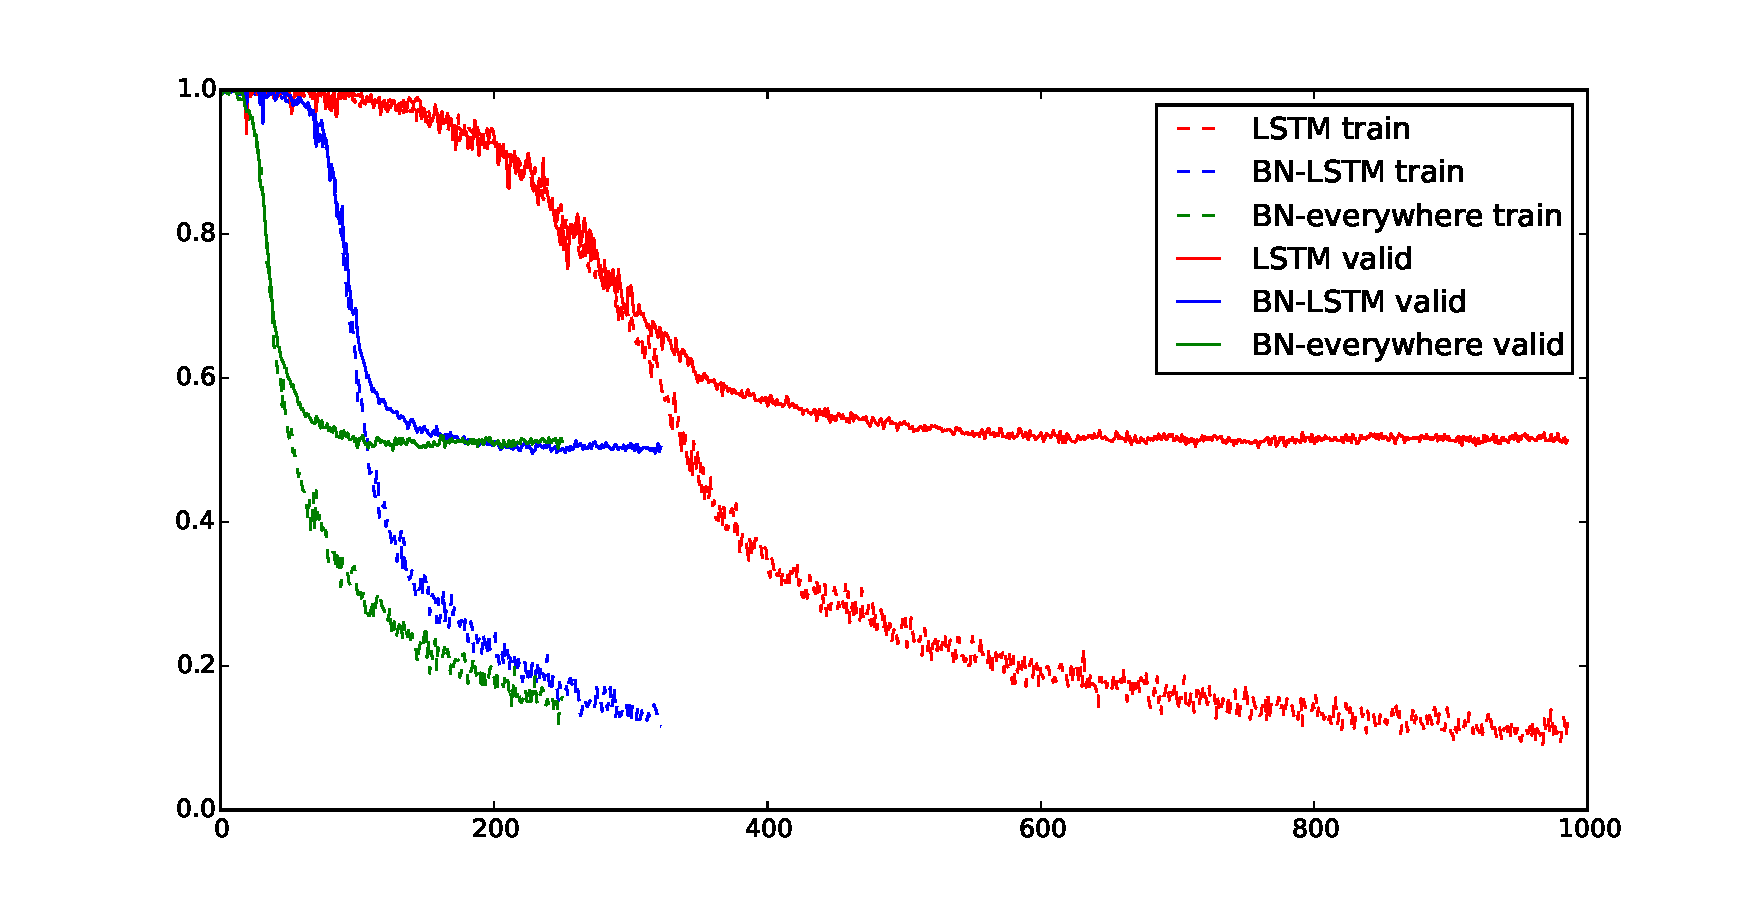
\includegraphics[width=0.95\textwidth]{figures/attr_valid.pdf}
\caption{
Error rate on the validation set for the Attentive Reader models on a variant of the CNN QA task~\cite{attentivereader}.
BN-LSTM converges much faster than the baseline LSTM.
Applying batch normalization in the attention computations as well (``BN-everywhere'') converges faster yet.
As detailed in the text, the theoretical lower bound on the error rate on this task is $43\%$.
}
\label{fig:attr_valid}
\end{figure}

To demonstrate the generality and practical applicability of our reparameterization,
we explore the use of batch-normalized LSTM in a unidirectional Attentive Reader Model~\cite{attentivereader}.
We evaluate two variants.
The first variant, referred to as BN-LSTM, consists of the vanilla Attentive Reader model with the LSTM simply replaced by our BN-LSTM reparameterization.
We further introduce batch normalization into the attention computations, normalizing each term going into the $\tanh$ nonlinearities, to obtain another variant which we term BN-everywhere.

All three variants are trained using the exact same hyperparameters.
The hidden state is composed of 240 units.
We use stochastic gradient descent on minibatches of size 64,
with gradient clipping at 10 and step rule determined by Adam~\cite{kingma2014adam}
with learning rate $8 \times 10^{-5}$.

We evaluate the Attentive Reader Model along with our batch-normalized variants on the question answering task using the CNN corpus, with placeholders to replace the named entities. We follow a similar preprocessing pipeline to~\cite{attentivereader}.
However contrary to~\cite{attentivereader}, we limit the number of sentences in each passage to 4 in order to save computation.
We choose which sentences to keep by performing a string matching between the question and the passage.
We rank the sentences in the text according to the string matching score and use only the top 4 sentences for each passage in the dataset.
The training, validation and test sets are all preprocessed using this same procedure.
After this procedure, the validation set has a recall of $57\%$ -- the passage contains the answer in only $57\%$ of the passage/question pairs.
This puts an upper bound on the accuracy that can be achieved.

During the training, we randomly sample the examples with replacement and shuffle the order of the placeholders in each text inside the minibatch. We use the whole vocabulary for the input and the answer which consists of 65829 unique words.

Figure~\ref{fig:attr_valid} shows the learning curves for the different variants of the attentive reader.
BN-LSTM trains dramatically faster than the LSTM baseline.
BN-everywhere, applying batch normalization in the attention computations as well, in turn shows a significant
improvement over BN-LSTM.
In addition, both BN-LSTM and BN-everywhere show a generalization benefit over the baseline.
We emphasize that these are preliminary results on the validation set; full results are forthcoming.

\section{Conclusion}

Contrary to previous findings~\cite{cesar,baidu},
we have demonstrated that batch-normalizing the hidden states of recurrent neural networks greatly improves optimization.
Indeed, doing so yields benefits similar to those of batch normalization in feed-forward neural networks:
our proposed BN-LSTM trains faster and generalizes better on a variety of tasks including language modeling and question-answering.
We have argued that proper initialization of the batch normalization parameters is crucial,
and suggest that previous difficulties~\cite{cesar, baidu} were due in large part to improper initialization.

\section*{Acknowledgements}

The authors would like to acknowledge the support of the following agencies for
research funding and computing support: the Nuance Foundation, Samsung, NSERC, Calcul Qu\'{e}bec, Compute Canada,
the Canada Research Chairs and CIFAR.
We thank the developers of Theano~\cite{theano2} and the
Blocks and Fuel~\cite{blocks} libraries for developing such powerful tools for scientific computing.
We further thank David Krueger, Saizheng Zhang, Ishmael Belghazi and Yoshua Bengio for discussions and suggestions.

\bibliography{index}
\bibliographystyle{nips2015}

\end{document}
